\subsection{Characterization of sub-wavelength grating}\label{sec:grating_characterization}

The sub-wavelength gratings, or Fano mirrors, used are commercially available high-quality silicone nitride $SiN$ membranes suspended on a $Si$ frame, which have been patterned into a grating. Figure \ref{fig:packaged_membrane} shows a packaged membrane from Norcada, which is the company who has provided all gratings/membranes used in this project. Figure \ref{fig:membrane_closeup} is a close-up picture of a bare membrane which have not yet been patterned, and includes a scale to provide perspective regarding the physical dimensions.

\begin{figure}[h!]
    \centering
    \begin{subfigure}[b]{0.35\textwidth}
        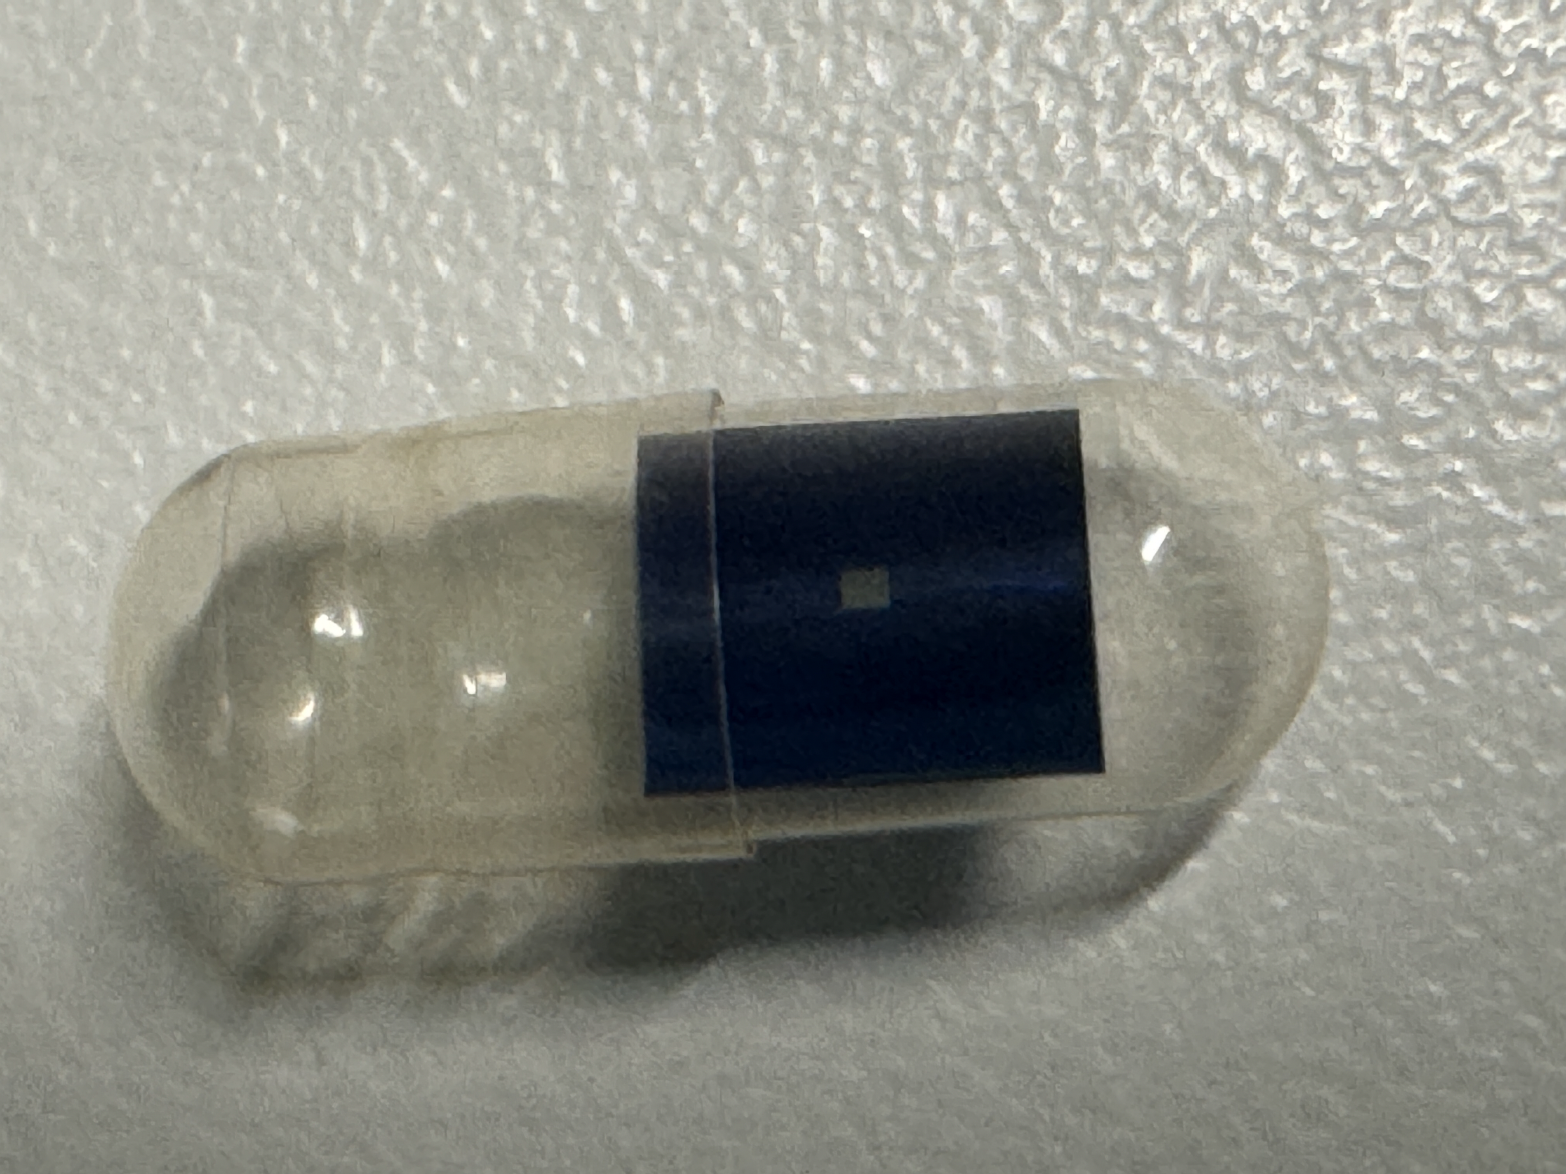
\includegraphics[width=\textwidth]{figures/packaged_membrane_picture.png}
        \caption{}
        \label{fig:packaged_membrane}
    \end{subfigure}
    \hspace{1cm}
    \begin{subfigure}[b]{0.35\textwidth}
        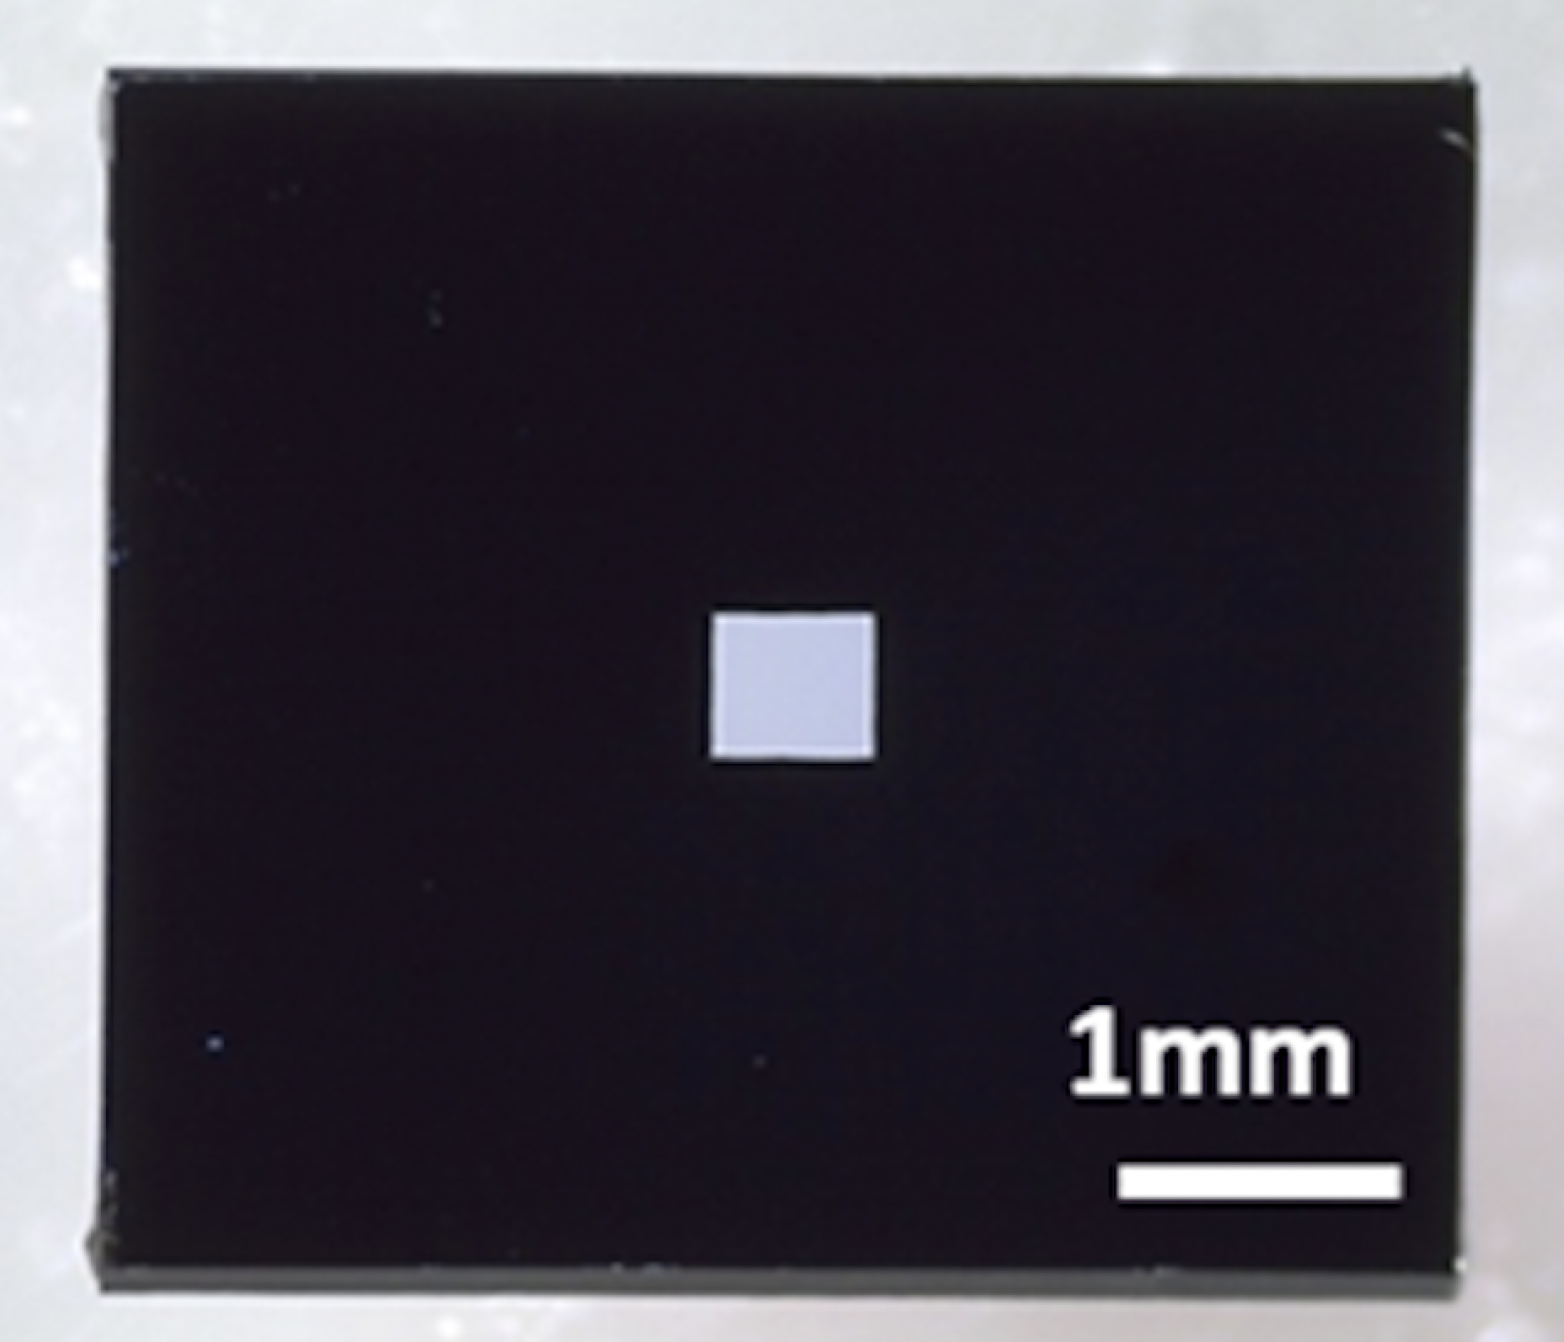
\includegraphics[width=\textwidth]{figures/membrane_picture.png}
        \caption{}
        \label{fig:membrane_closeup}
    \end{subfigure}
    \caption{(a) shows an image of a packaged bare membrane, which has not yet been patterned, from Norcada. (b) is a close-up image of a bare membrane like the one in figure \ref{fig:packaged_membrane}.}
    \label{fig:membrane_pictures}
\end{figure}

The patterned area of the Fano mirrors used throughout this project is $400$ x $400 \mu m$, and this along with detailed dimensions of the whole membrane is sketched in figure \ref{fig:grating_sketch}.

\begin{figure}[h!]
    \centering
    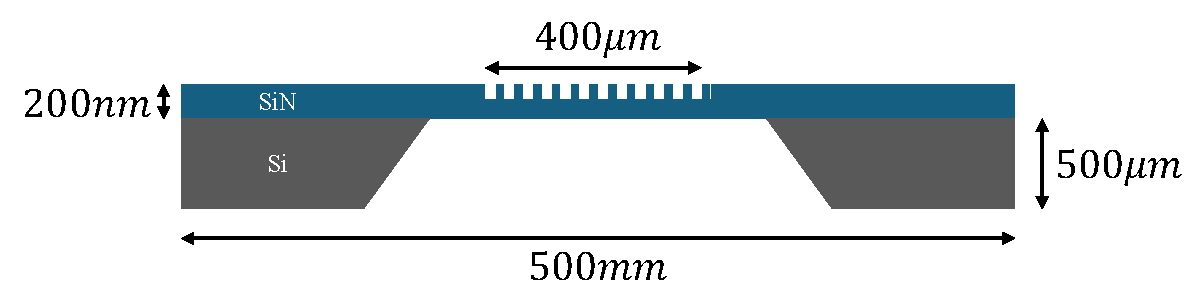
\includegraphics[width=0.6\textwidth]{figures/grating_sketch.pdf}
    \caption{A simple sketch of the profile of a patterned membrane, i.e. a Fano mirror. It is seen that the width of the patterned area is $400\mu m$.}
    \label{fig:grating_sketch}
\end{figure}

\subsubsection{The alignment procedure}\label{sec:alignment}

In order to align the Fano mirror for its optical characterization only, the setup utilized is a simplified one, compared with the double Fano cavity setup shown in figure \ref{fig:setup_zoomed}. This setup corresponds to one where only the \emph{bottom} part is included, i.e. corresponding to the one highlighted in figure \ref{fig:setup_bottom}. It must here be noted, that if the purpose of the Fano mirror alignment is to create a cavity, the top part shown in figure \ref{fig:setup_top} must of course be utilized as well. 

The goal of the alignment procedure is to ensure that the coupling between the guided-mode and the mode of the laser is maximized, this is outlined in section \ref{sec:fano_mirror}. The transmission of the Fano mirror is measured during alignment with a \emph{PM100D} digital handheld optical power meter from Thorlabs, and progression of the alignment procedure is understood as minmizing the transmission. The behavior of the Fano mirror transmission, when perfectly aligned, can be seen in figure \ref{fig:lossy_grating_spectrum}, where it has been simulated for a Fano mirror of arbitrary parameters. When aligned, the guided-mode resonance wavelength can thus be found. This is practically done by scanning the expected wavelength range using the Toptica laser and recording the wavelength at which the transmission is minimized.  

The three degrees of freedom, in which the alignment of the Fano mirror is optimized, are the spacial coordinates ($x$, $y$), the rotational degree of freedom, and the two angular degrees of freedom. It is assumed at this point that the waist of the beam incident on the Fano mirror is optimal, this will be expanded upon in section \ref{sec:beam_waist}.

The general order in which the alignement is done is given as:
\begin{enumerate}
    \item xy-plane alignment. 
    \item Alignment of the angular degrees of freedom (adjusting the kinematic mirror mount).
    \item Rotational alignment (adjusting the HWP placed prior to the cavity setup).
\end{enumerate}

\subsubsection*{xy-plane alignment}
The spacial alignement of the Fano mirror in the xy-plane is simply done by movement of the xy-stages (linear $\mu m$-stages from Thorlabs) shown in figure \ref{fig:setup_zoomed}. Here it is crucial to know how the transmission level behaves qualitatively as a function of the xy-positions when the wavelength of the laser is off-resonance with respect to the guided-mode of the Fano mirror. Due to the effective thickness of the membrane in patterned and un-patterned areas being different, the transmission properties will vary slightly. This can be utilized in order to align these parameters effectively. Assuming one of the coordinates, $x$ or $y$, is optimal, and one scans across the other as indicated in figure \ref{fig:xy_alignment_sketch}, it will be evident that the transmission is constant when the entire beam is incident on the bare membrane, while it will experience a slight decrease in the patterned area, simply due to the lower effective thickness of the structure in this area. For this reason the optimal alignment in this direction is found as the minimum transmission as a function hereof. 

\begin{figure}[h!]
    \centering 
    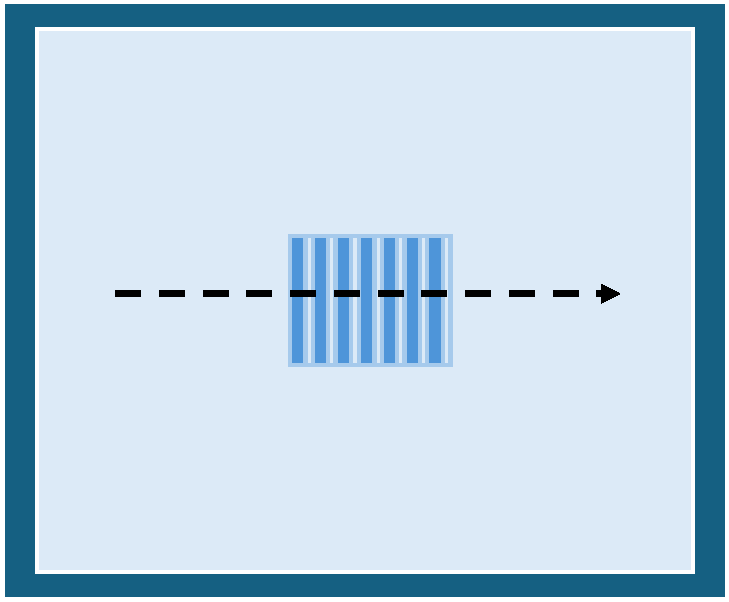
\includegraphics[width=0.3\textwidth]{figures/xy_alignment_sketch.pdf}
    \caption{Simple sketch of a patterned membrane, i.e. a Fano mirror. The darker area surrounding the $SiN$ membrane is the $Si$ frame and the dark blue lines in the center indicate the $400$ x $400 \mu m$ patterned area. The black dotted arrow is indicative of scanning across the membrane, by moving it relative to the beam, using one of the linear stages.}
    \label{fig:xy_alignment_sketch}
\end{figure}

\subsubsection*{Angular alignment}
Adjusting the angular alignment, which is done by adjusting the screws on the kinematic mirror mount holding the piezo ring and the Macor membrane holder, is crucial for the evaluation of the guided-mode resonance wavelength. As reported by Parthenopoulos et al. in \cite{Parthenopoulos} the resonance wavelength of the guided-mode depends strongly on the angle of incidence. 

In figure \ref{fig:setup_sketch} the components $I_{1-4}$ indicate apertures (iris') used for the angular alignment. Specifically $I_1$ and $I_2$ are used to track the back-reflection of the beam incident on the Fano mirror to ensure a high degree of overlap as possible. A complete overlap indicates that the incident beam is normal to the Fano mirror surface. 

\subsubsection*{Rotational alignment}
The Fano mirrors provided by Norcada are of so-called TM polarization, meaning that the magnetic field is parallel to the grating lines, and is thus perpendicular to the electric field. Since the polarization is defined along the axis of the electric field, this means that the polarization axis must also be perpendicular to the grating lines, as this ensures the interaction is maximized\cite{Sadov}.

For this reason the rotational alignment is vital to achieving the correct minimum transmission wavelength of the Fano mirror. 

Since no rotaitonal degree of freedom is appointed the Fano mirror itself, and that this would greatly complicate the alignment procedure, the rotational alignment is achieved by changing the polarization of the incident light. This done by adjusting hte rotating HWP placed immediately before the light hits the Fano mirror surface and is possible due to its effect on linearly polarized light illustrated in figure \ref{fig:HWP}.

\subsubsection{Adjusting and measuring the beam waist - the razor blade method and the optical telescope}\label{sec:beam_waist}

In section \ref{sec:alignment} we assumed an optimal beam waist as the alignment procedure was outlined. This was due to the fact that the beam waist optimization is unecessary unless the entire setup is rebuilt or if the size of the Fano mirror is changed. Since the patterned area of the Fano mirrors characterized in this project was only $400$ x $400 \mu m$, the beam waist optimization was only done once.

As is evident from figure \ref{fig:telescope} how an optical telecope was utilized to tune the waist size $w_0$ of the collimated laser beam. In order to determine the optimal value of $w_0$ the second lens $L_2$ was moved back and forth without diverging from the position where the optical axis passed through the center of the lens. The minimum transmission was recorded for each iteration, and the transmission would converge towards its minimum value (or at least the lowest achievable value). When the mininum transmission as a function of $w_0$ was found, this was recorded using the \emph{razor blade method}. The razor blade method is a simple tool to, fairly accurately, measure the beam waist of a Gaussion laser beam by \emph{cutting} the beam gradually with a razor blade. The distance the razor blade moves is recorded along with the transmitted intensity, and the two are thus directy correlated\cite{Forster}.

An arbitrary Gaussian distribution, corresponding to a laser beam in the TEM00 mode, is shown on the left in figure \ref{fig:razor_blade_method}, while the right plot shows the integral of the distribution as a function of the razor blade position. 

\begin{figure}[h!]
    \centering
    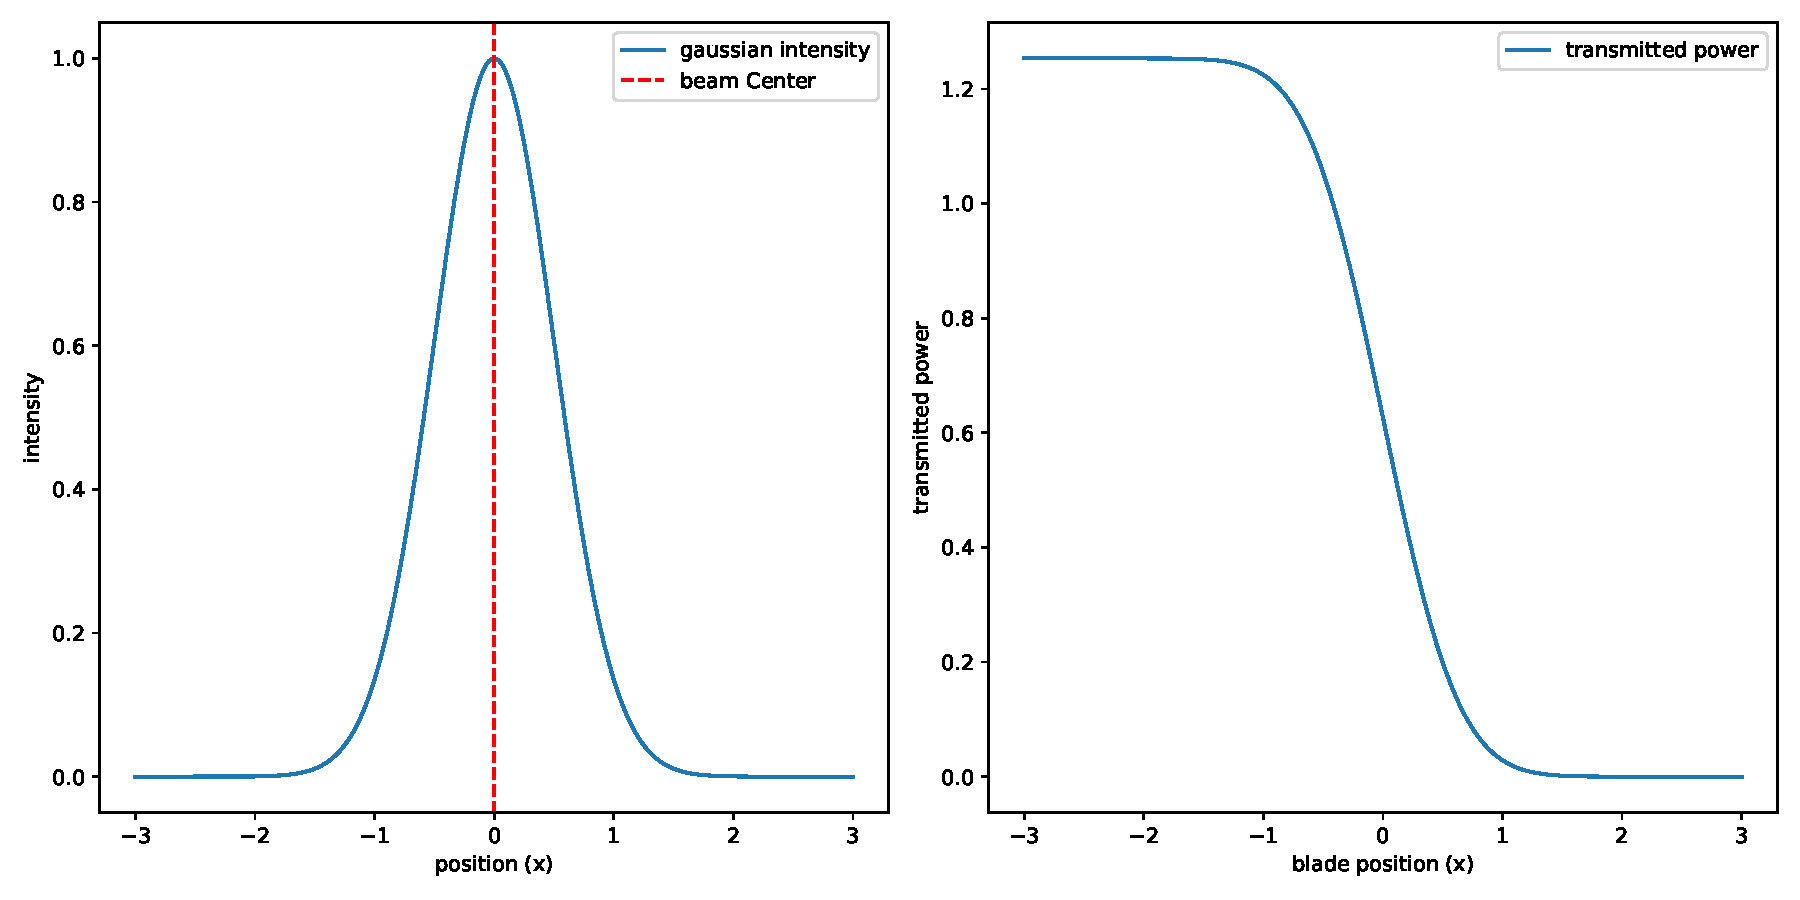
\includegraphics[width=0.8\textwidth]{figures/razor_blade_method.pdf}
    \caption{The left plot shows an arbitrary Gaussian distribution, and the red dashed line indicate the placement of the maximum value. The right plot shows the transmitted intensity as a function of the position of the razor blade, as the razor blade method is simulated, i.e. the beam is gradually covered with the blade.}
    \label{fig:razor_blade_method}
\end{figure}

In practice the blade position was recorded by counting the turns made on a linear $\mu m$-stage with the razor blade attached, and the transmitted intensity was recorded live by a power meter from Thorlabs. The power of the laser beam without being \emph{cut} by the blade was tuned to $\sim 1 mW$ such that the percentile change was intuitively seen. The linewidth of the Gaussion beam is then approximately given as the distance between the two cut-off points where the transmitted intensity is given as $16\%$ and $84\%$\footnote{In reality this interval corresponds to the width according to two standard deviations $2\sigma$, which is only approximately equal to the linewidth.}. The optimal value for the linewidth was found to be
\begin{equation}
    \delta \lambda_{400 \mu m} \approx 160 \mu m.
\end{equation}

\subsubsection{Obtaining normalized transmission/reflection spectra}



\subsubsection{Normalization}

% finding a match (include either as a section or as part of one)
